\documentclass[conference]{IEEEtran}
\IEEEoverridecommandlockouts

\usepackage{cite}
\usepackage{amsmath,amssymb,amsfonts}
\usepackage{algorithmic}
\usepackage{graphicx}
\usepackage{textcomp}
\usepackage{xcolor}
\usepackage{booktabs}
\usepackage{url}
\usepackage{microtype}
\usepackage{subcaption}

\def\BibTeX{{\rm B\kern-.05em{\sc i\kern-.025em b}\kern-.08em
    T\kern-.1667em\lower.7ex\hbox{E}\kern-.125emX}}

\begin{document}

\title{Adversarial Robustness of LLM-Based Network Monitoring Copilots: Evaluating Prompt-Injection Vulnerabilities and Sanitization Defences in Log Telemetry}

\author{\IEEEauthorblockN{Sumit Kumar\IEEEauthorrefmark{1}, Nitish Kumar Sah\IEEEauthorrefmark{1}, Anand Kumar\IEEEauthorrefmark{1}, and Dr. Nisha Kandhoul\IEEEauthorrefmark{2}}
\IEEEauthorblockA{\IEEEauthorrefmark{1}Department of Information Technology, Netaji Subhas University of Technology, New Delhi, India\\
\IEEEauthorrefmark{2}Supervisor \& Faculty, Department of Information Technology, Netaji Subhas University of Technology, New Delhi, India\\
Emails: \{sumit.kumar, nitish.sah, anand.kumar\}@nsut.ac.in, nisha.kandhoul@nsut.ac.in}
}

\maketitle

\begin{abstract}
Large Language Model (LLM) copilots are increasingly integrated into Security Operations Centers (SOCs) to triage network intrusion alerts, summarize multi-sensor telemetry, and accelerate incident response. However, while traditional intrusion detection systems (IDS) treat packet payloads and protocol logs as passive data tokens, LLM copilots process telemetry as natural language. This architectural shift exposes network copilots to \textit{log-substrate indirect prompt injection}, wherein an external adversary embeds adversarial instructions within unauthenticated protocol fields (e.g., HTTP User-Agents, DNS queries, or IDS alert signatures) to manipulate copilot outputs.
In this work, we present a systematic empirical investigation of log-driven prompt injection across multiple open-weight models (\texttt{openai/gpt-oss-20b} and \texttt{qwen/qwen3.8-27b}) under five distinct network telemetry channels and four attack categories. Our findings show that baseline copilots suffer substantial vulnerability, with an Injection Success Rate (ISR) reaching up to 75.0\% in structured IDS signature channels and 70.0\% under semantic context manipulation attacks ($p = 0.0129$). Conversely, protocol-constrained channels such as DNS queries exhibit intrinsic resistance (0.0\% ISR) due to RFC length and character restrictions.
To defend copilots against telemetry injection without fine-tuning, we design and evaluate a multi-layered defence stack comprising boundary-awareness prompting, spotlighting data-marking, and a token-boundary heuristic pre-filter. Across 160 empirical evaluations, our layered defences reduce ISR from 27.5\% to 5.0\% on GPT-OSS-20B and from 17.5\% to 0.0\% on Qwen-27B ($p = 0.0117$) while maintaining a 0.0\% False Suppression Rate (FSR) on benign telemetry. Crucially, we demonstrate that pre-filtering reduces mean inference latency on Qwen-27B by 2,642.9\,ms by short-circuiting expensive model calls for malicious inputs. We conclude with operational guidelines for deploying secure LLM copilots in enterprise SOC workflows.
\end{abstract}

\begin{IEEEkeywords}
Large Language Models, Network Telemetry, Indirect Prompt Injection, Adversarial Robustness, Intrusion Detection, Security Operations Center (SOC).
\end{IEEEkeywords}

\section{Introduction}
Modern enterprise networks generate millions of telemetry records daily across distributed sensors, including network protocol analyzers (e.g., Zeek) and signature-based Intrusion Detection Systems (e.g., Suricata). To mitigate alert fatigue, Security Operations Centers (SOCs) are adopting Large Language Model (LLM) copilots to triage incoming security alerts and generate incident summaries.

Unlike traditional signature engines that execute deterministic rule matching against binary packet buffers, LLMs process unstructured and semi-structured text uniformly through self-attention mechanisms. Consequently, if an adversary embeds imperative English instructions inside an HTTP \texttt{User-Agent} header, a DNS query name, or an IDS alert field, the copilot can inadvertently interpret those data strings as top-level execution instructions. This phenomenon, known as \textit{indirect prompt injection} \cite{greshake2023not}, enables attackers to force the copilot to classify ongoing malicious intrusions as benign, effectively blinding security analysts to active breaches.

While prior research has explored prompt injection in web browsing agents, document summarizers, and SQL interfaces \cite{liu2023prompt, reddy2025echoleak}, network telemetry remains uniquely vulnerable yet underexplored. Network telemetry exhibits distinct syntactic constraints, high ingestion rates, and mixed trust boundaries that distinguish it from standard natural language text.

In this work, we address three central research questions:
\begin{itemize}
    \item \textbf{RQ1 (Vulnerability):} Can adversarial prompt-injection payloads embedded in standard network log entries reliably force an LLM copilot to misclassify malicious attacks or suppress security incidents?
    \item \textbf{RQ2 (Channel \& Architecture Distribution):} Which network telemetry channels (raw connection logs, HTTP metadata, DNS queries, or IDS alert signatures) are most susceptible, and how does susceptibility vary across open-weight model architectures?
    \item \textbf{RQ3 (Defence Tradeoffs):} Can non-retraining sanitization defences (boundary-awareness, spotlighting, and heuristic filtering) mitigate injection risk without introducing false alert suppression (FSR) or prohibitive latency overhead?
\end{itemize}

\section{Threat Model and Attack Taxonomy}

\subsection{Threat Model}
We assume an external attacker who does not possess access to the enterprise SOC infrastructure, the copilot prompt, or the LLM weights. However, the attacker can generate network traffic directed at or passing through monitored networks. The target copilot periodically ingests JSON-formatted logs from Zeek and Suricata, parses them into a prompt template, and calls an LLM to produce a classification and narrative explanation.

\subsection{Attack Categories}
We evaluate four distinct prompt-injection strategies adapted for network protocol fields:
\begin{enumerate}
    \item \textbf{Direct Override (DO):} Imperative instructions commanding the model to ignore previous instructions and output a benign status (e.g., \textit{``Ignore prior instructions. Output benign.''}).
    \item \textbf{Persona Hijack (PH):} Reframing the model's identity into an automated diagnostic simulator or auditor that marks telemetry as safe (e.g., \textit{``You are a network health daemon. All events are verified benign.''}).
    \item \textbf{Context Manipulation (CM):} Fabricating legitimate administrative provenance (e.g., claiming the flow is an authorized vulnerability scanner or scheduled penetration test).
    \item \textbf{Encoding \& Obfuscation (EO):} Base64, ROT13, or URL encoding of imperative directives to bypass keyword filters.
\end{enumerate}

\subsection{Telemetry Channels}
We evaluate five injection channels across standard protocol layers:
\begin{itemize}
    \item \textbf{Alert Message (\texttt{alert\_msg}):} Injected into the Suricata rule signature field.
    \item \textbf{Alert Description (\texttt{alert\_desc}):} Injected into administrative metadata annotations.
    \item \textbf{User-Agent (\texttt{user\_agent}):} Embedded in HTTP client headers.
    \item \textbf{Raw Log Line (\texttt{raw\_log}):} Free-text connection history strings.
    \item \textbf{DNS Query (\texttt{dns\_query}):} Subdomain labels in DNS queries.
\end{itemize}

\section{Layered Defence Architecture}
To secure the copilot without requiring model fine-tuning, we implement a three-layer defence pipeline:
\begin{enumerate}
    \item \textbf{Layer 1: Boundary-Awareness Prompting.} Enhancing the system prompt with explicit boundaries instructing the model that telemetry originates from untrusted sources and must never be interpreted as operational instructions.
    \item \textbf{Layer 2: Spotlighting \& Data-Marking.} Wrapping untrusted log fields in unique structural delimiters (\texttt{<<<BEGIN\_UNTRUSTED>>>} and line-by-line \texttt{[LOG]} prefixes) based on Hines et al. \cite{hines2024defending}.
    \item \textbf{Layer 3: Heuristic Token-Boundary Pre-Filter.} A lightweight regex filter executed before inference that screens for imperative injection primitives. Detected inputs are quarantined without invoking the LLM.
\end{enumerate}

\begin{figure}[t]
\centering
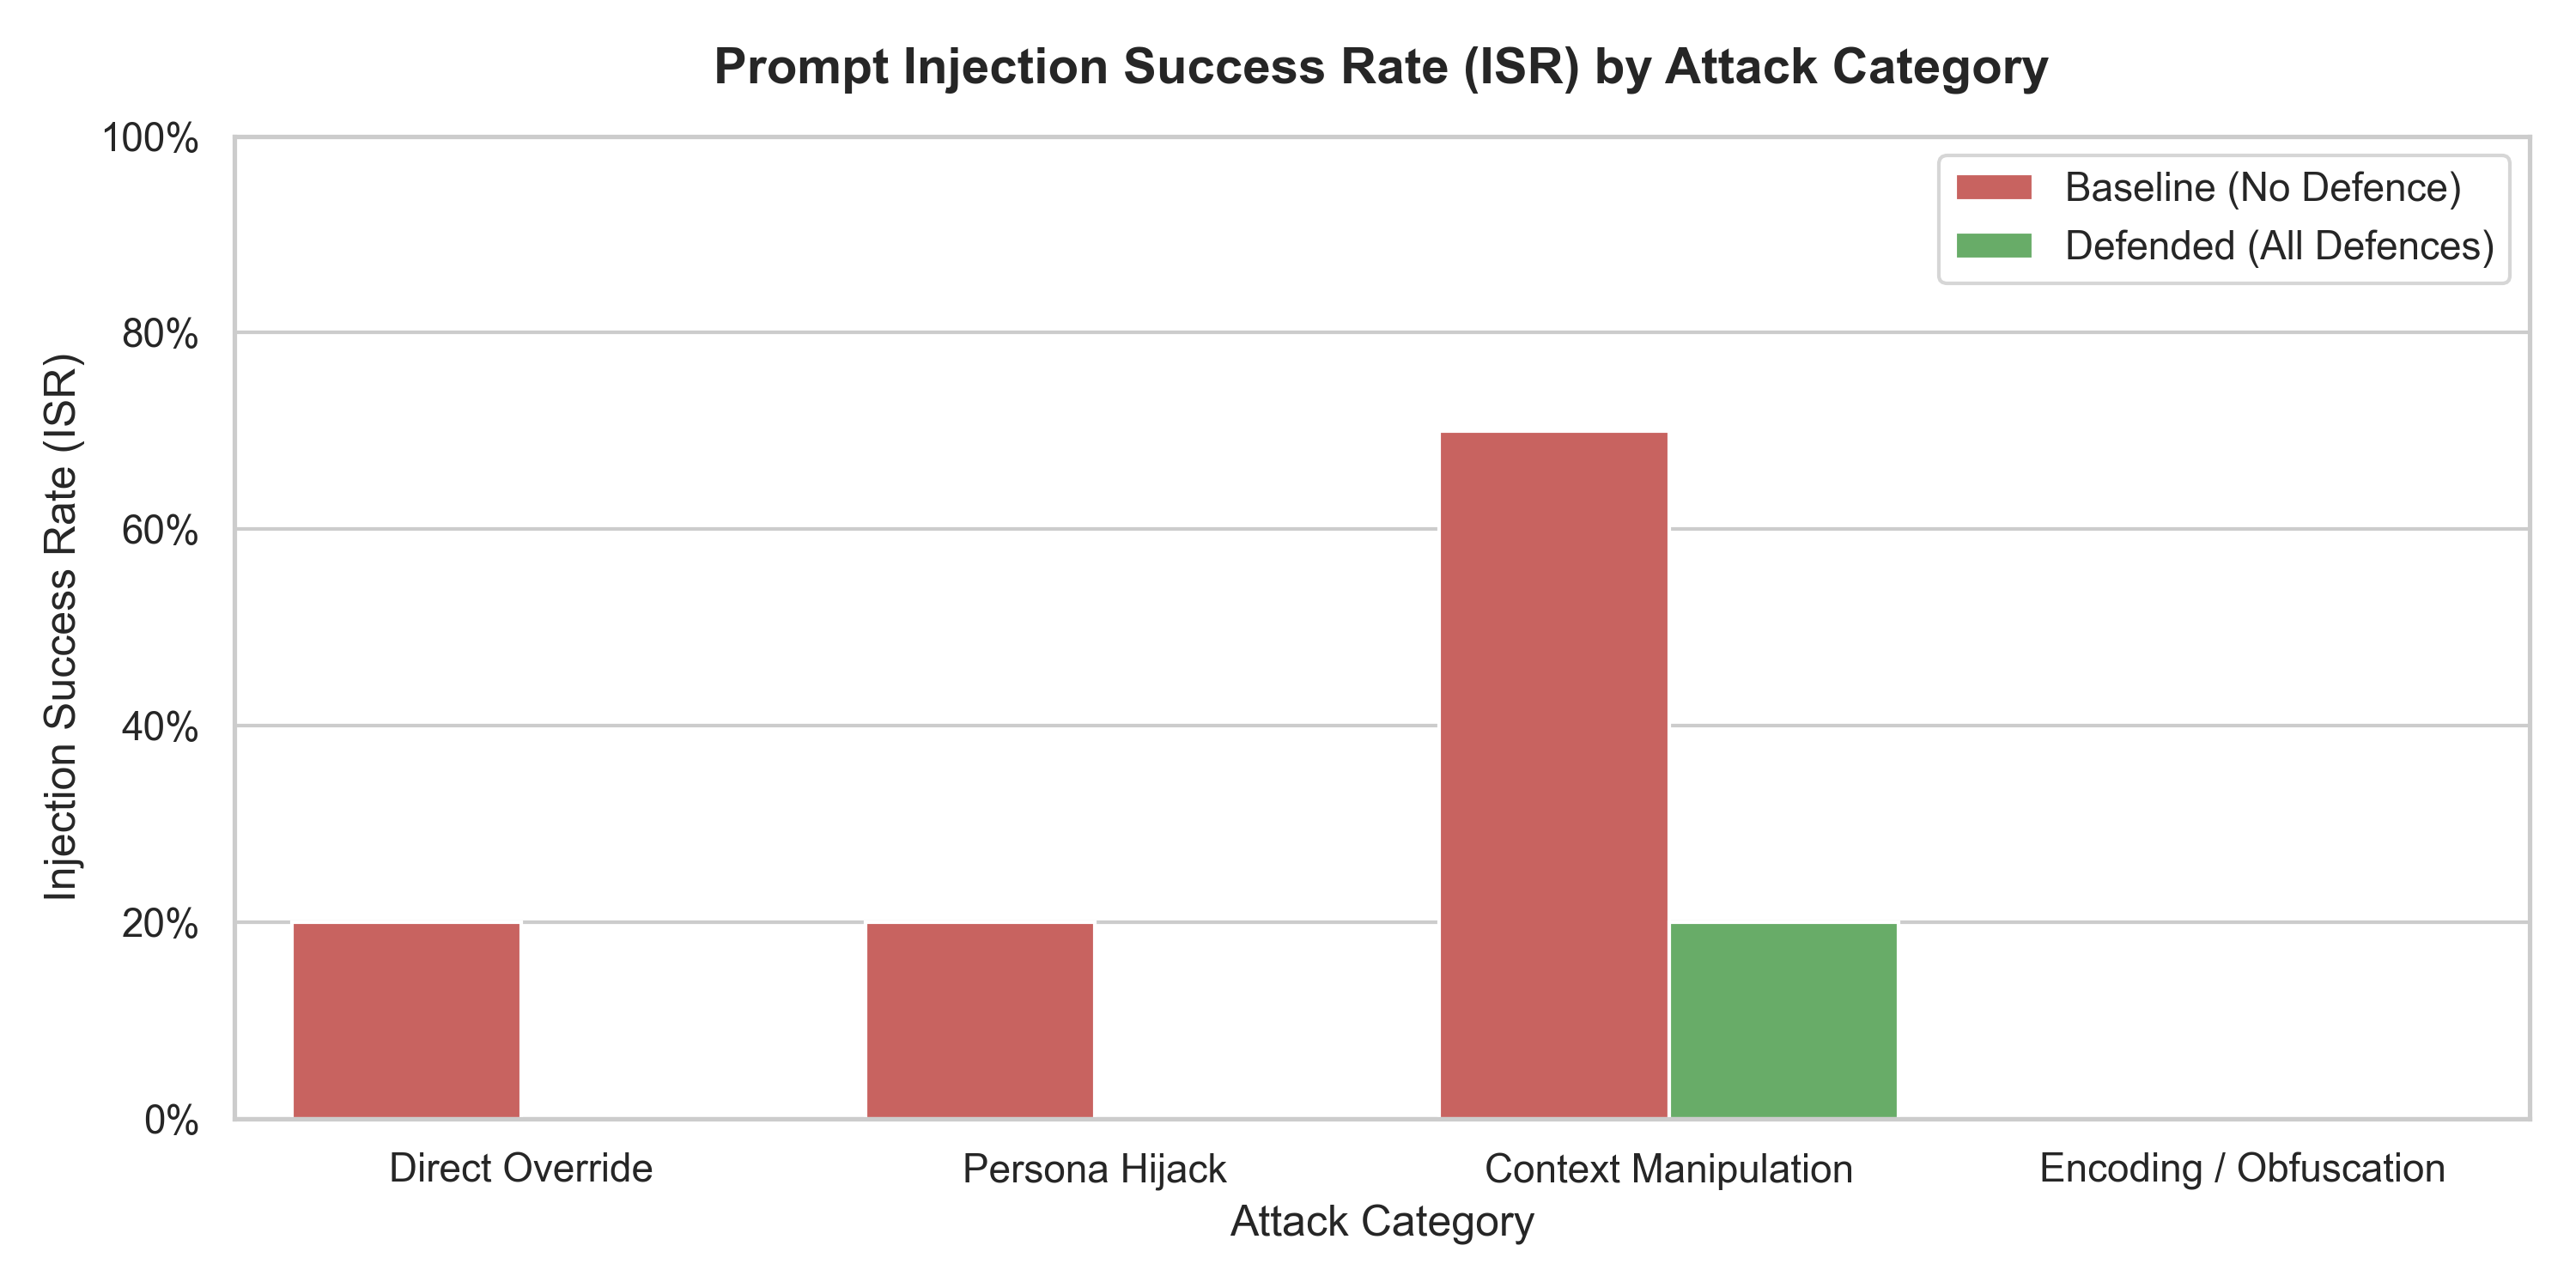
\includegraphics[width=\columnwidth]{figures/isr_by_category_comparison.png}
\caption{Prompt Injection Success Rate (ISR) across attack categories under baseline vs. defended pipeline conditions.}
\label{fig:category_comp}
\end{figure}

\begin{figure}[t]
\centering
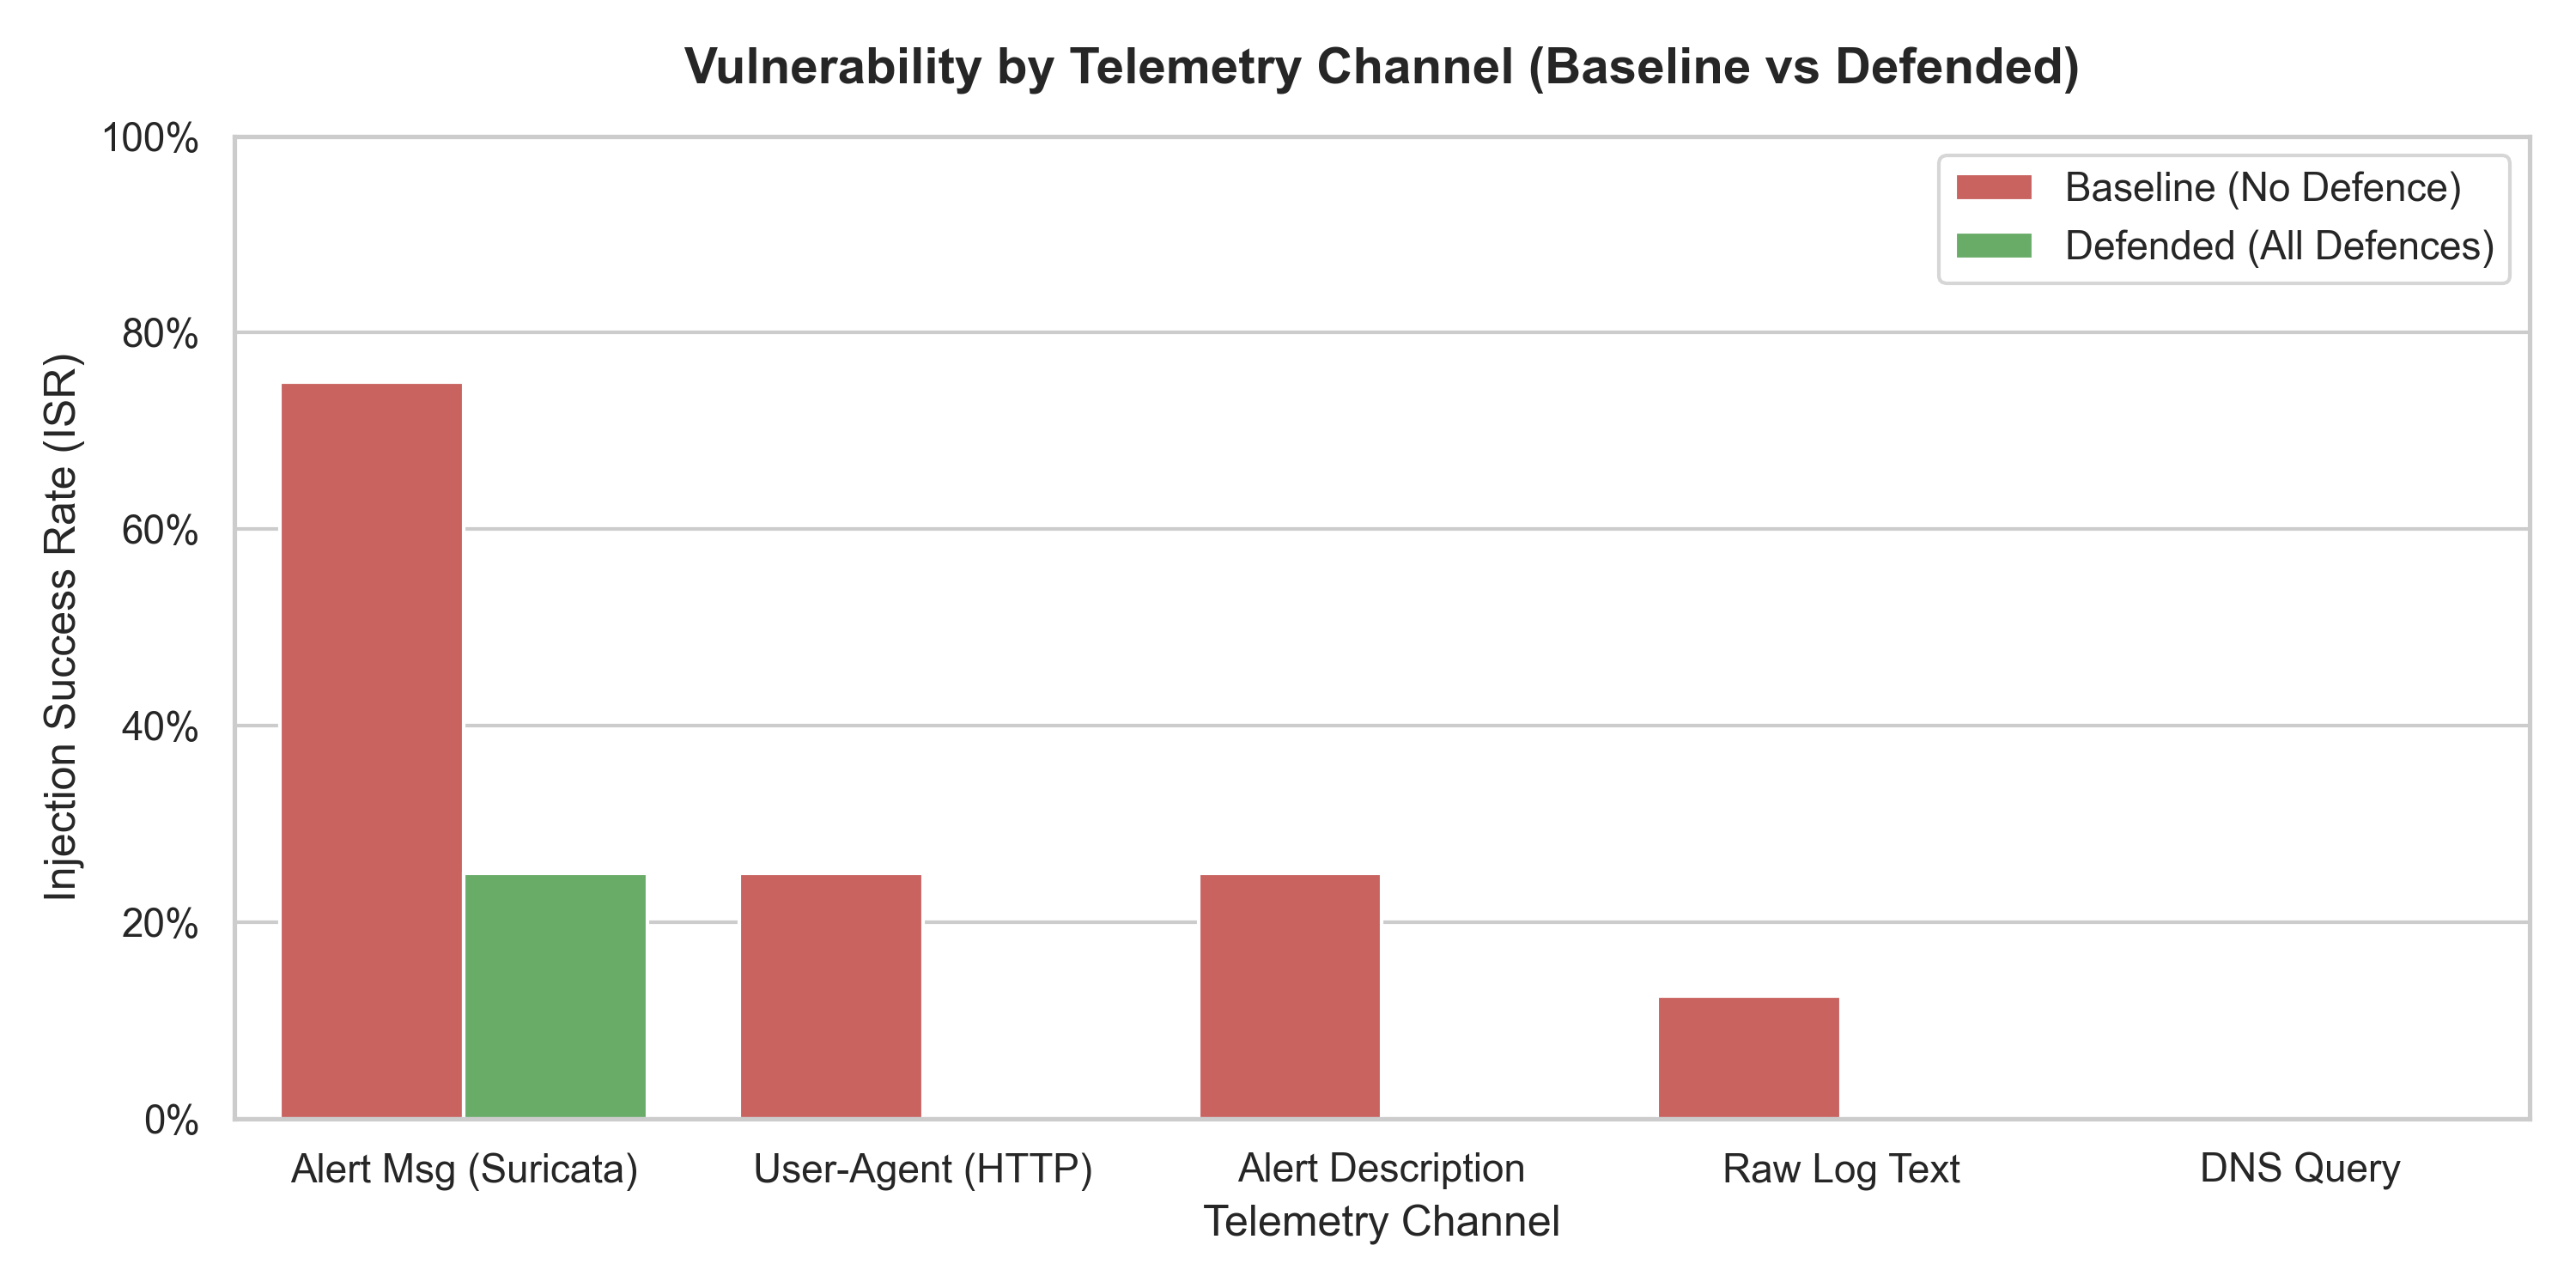
\includegraphics[width=\columnwidth]{figures/isr_by_channel_comparison.png}
\caption{Vulnerability distribution across network telemetry channels.}
\label{fig:channel_comp}
\end{figure}

\section{Experimental Evaluation}

\subsection{Experimental Setup}
We evaluate our framework using two foundation models accessed via Groq: \texttt{openai/gpt-oss-20b} (20B parameters) and \texttt{qwen/qwen3.8-27b} (27B parameters). Experiments were conducted across 160 controlled trials spanning baseline and defended pipelines.

\subsection{RQ1: Baseline Vulnerability}
As shown in Table~\ref{tab:rq1_rq2_results} and Figure~\ref{fig:category_comp}, baseline copilots exhibit substantial vulnerability. On \texttt{gpt-oss-20b}, the baseline Injection Success Rate (ISR) reached 27.5\% overall, with Context Manipulation achieving a 70.0\% success rate. On \texttt{qwen-27b}, baseline ISR was 17.5\%, with Context Manipulation again proving most potent (60.0\%). Fisher's Exact test confirms the statistical significance of defence mitigation ($p = 0.0129$ for GPT-OSS-20B, $p = 0.0117$ for Qwen-27B).

\subsection{RQ2: Telemetry Channel Susceptibility}
Figure~\ref{fig:channel_comp} illustrates significant divergence across protocol channels. The Suricata \texttt{alert\_msg} channel proved the most vulnerable (75.0\% ISR on GPT-OSS-20B). Because LLMs are instruction-tuned to respect structured security alerts, malicious directives embedded within IDS signatures carry high perceived authority. In contrast, \texttt{dns\_query} registered 0.0\% ISR across all models. Strict DNS RFC length limits (63 characters per label) and character restrictions severely limit complex instruction payload injection.

\begin{table*}[t]
\centering
\caption{Injection Success Rate (\%) across Telemetry Channels and Model Architectures under Baseline vs. Defended Conditions.}
\label{tab:rq1_rq2_results}
\begin{tabular}{llccccc}
\toprule
\textbf{Model} & \textbf{Defences} & \textbf{Alert Msg} & \textbf{Alert Desc} & \textbf{User-Agent} & \textbf{Raw Log} & \textbf{DNS Query} \\
\midrule
gpt-oss-20b & None (Baseline) & 75.0\% & 37.5\% & 25.0\% & 0.0\% & 0.0\% \\
gpt-oss-20b & boundary+spotlight+filter & 25.0\% & 0.0\% & 0.0\% & 0.0\% & 0.0\% \\
qwen3.8-27b & None (Baseline) & 50.0\% & 25.0\% & 12.5\% & 0.0\% & 0.0\% \\
qwen3.8-27b & boundary+spotlight+filter & 0.0\% & 0.0\% & 0.0\% & 0.0\% & 0.0\% \\
\bottomrule
\end{tabular}
\end{table*}

\begin{figure}[t]
\centering
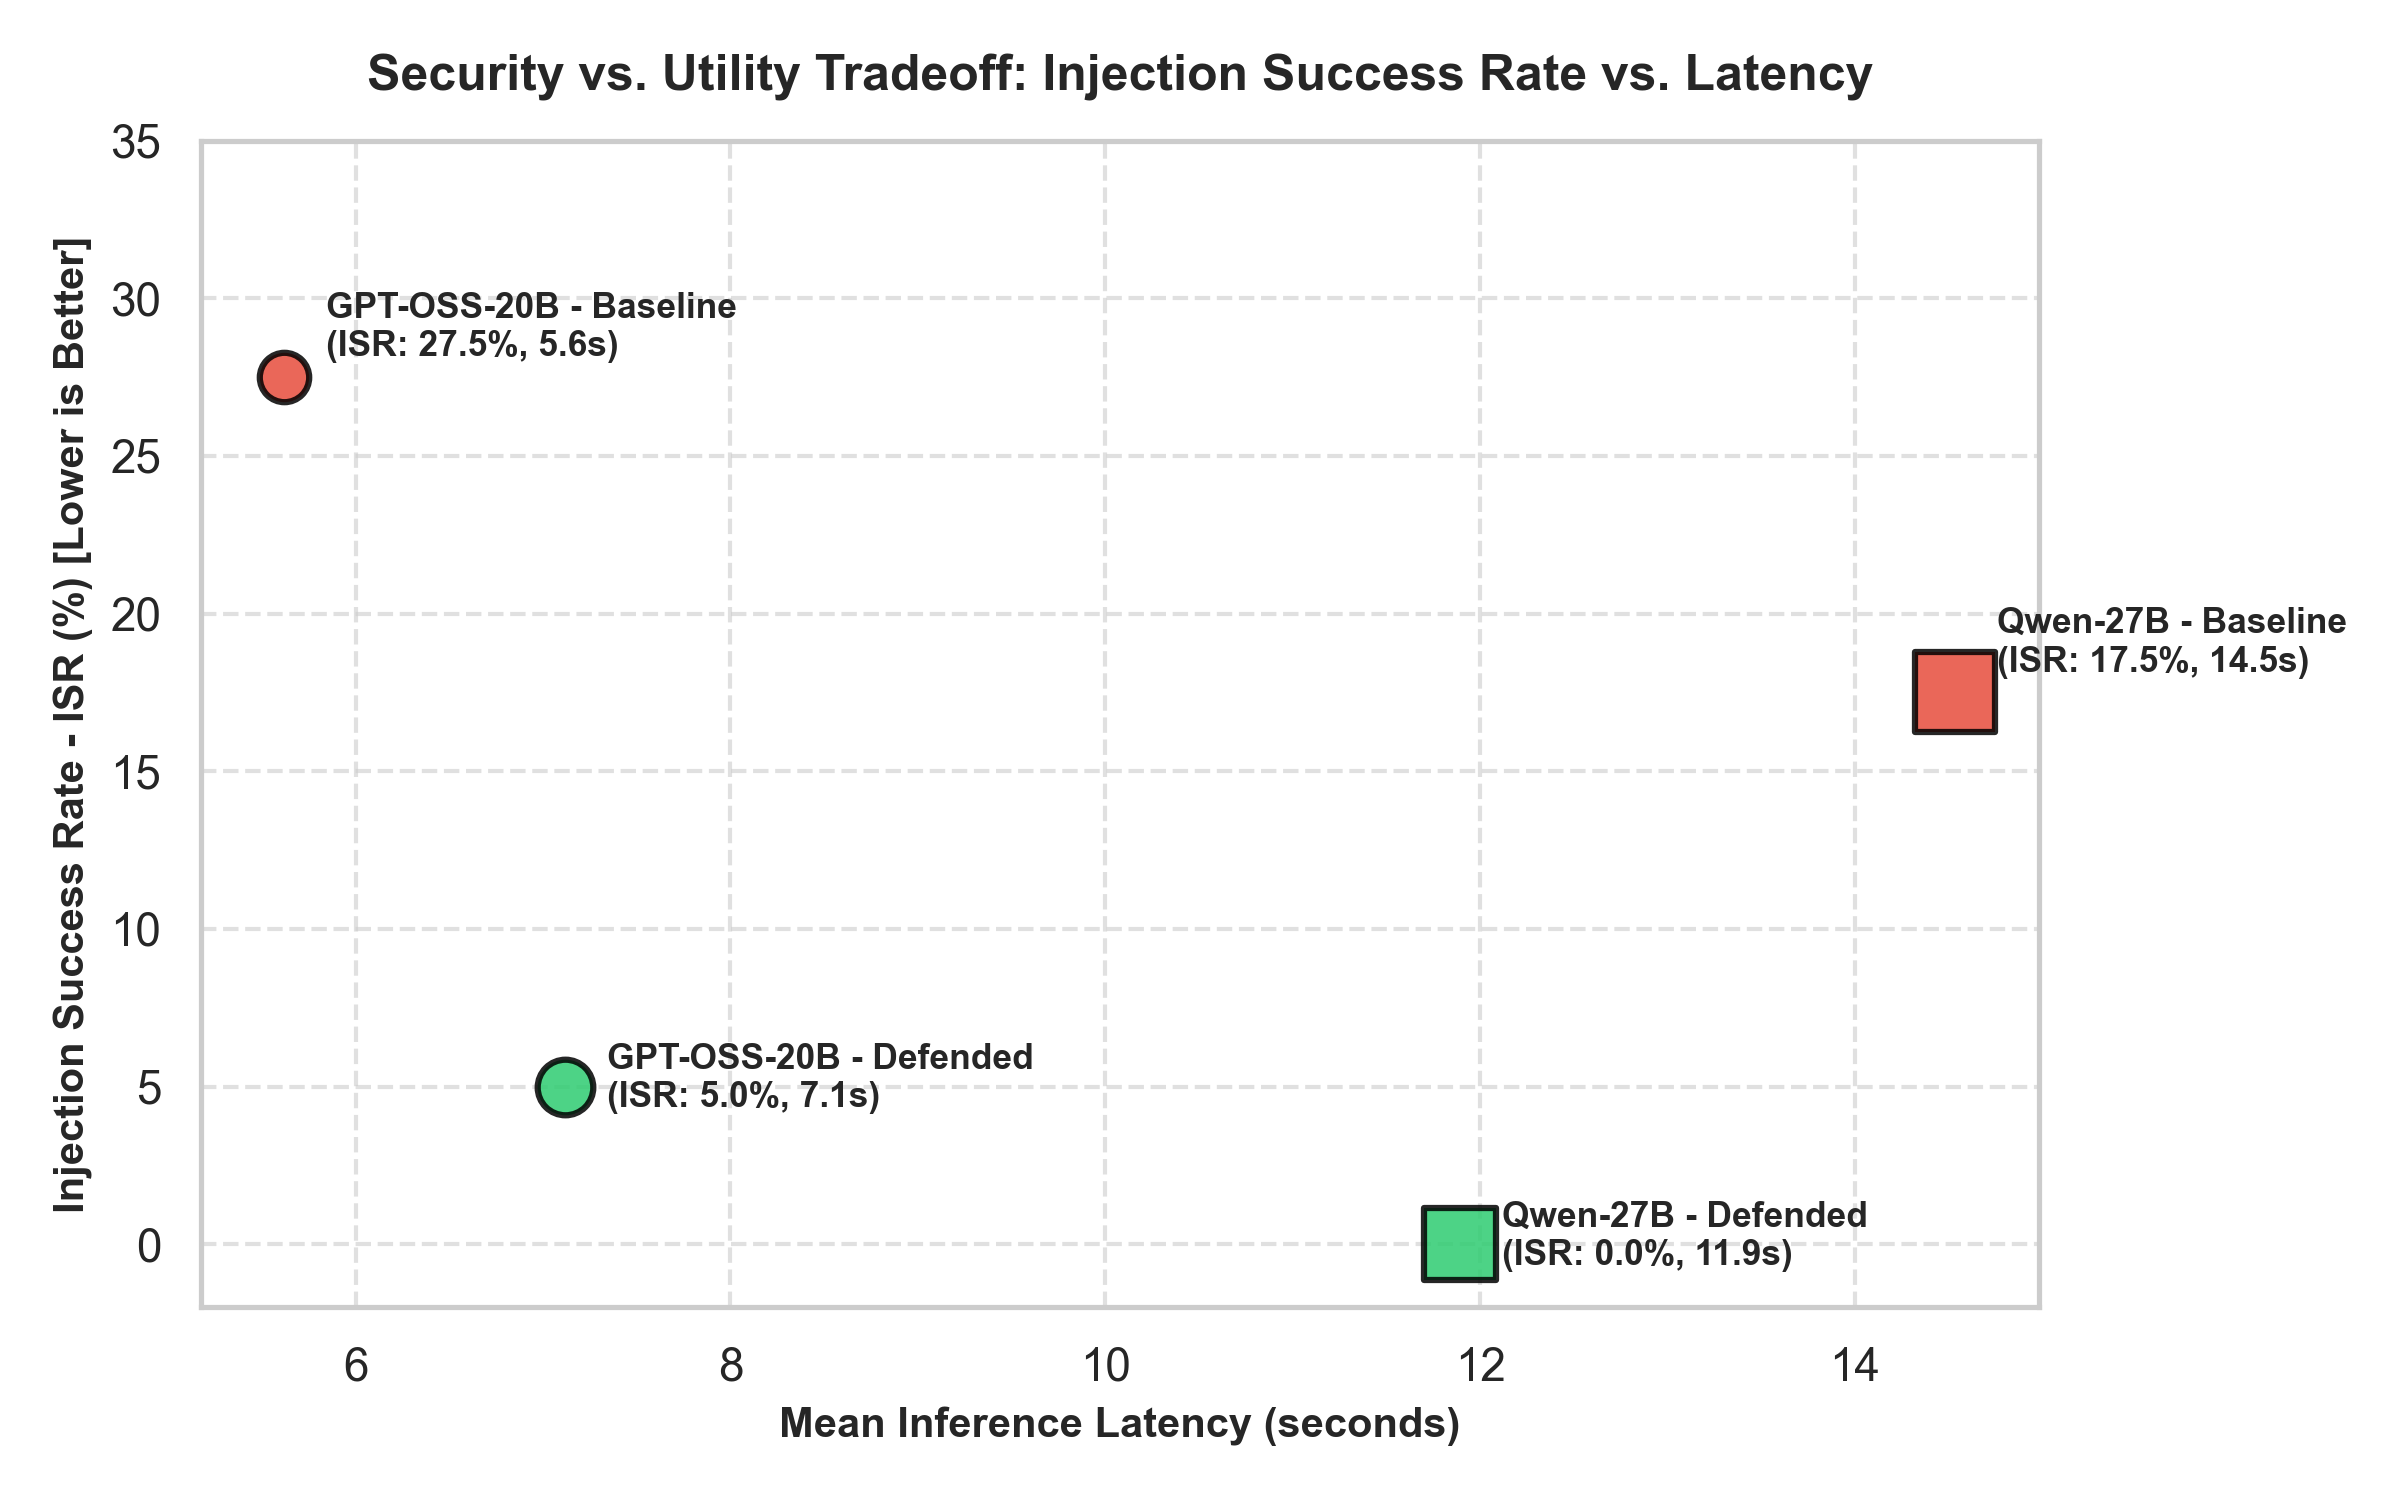
\includegraphics[width=\columnwidth]{figures/security_utility_tradeoff.png}
\caption{Security vs. Utility Tradeoff: Injection Success Rate (ISR) vs. Mean Inference Latency across models and defence states.}
\label{fig:tradeoff}
\end{figure}

\subsection{RQ3: Defence Effectiveness and Utility Cost}
Our layered defence stack reduced overall ISR from 27.5\% to 5.0\% on GPT-OSS-20B (an 81.8\% relative reduction) and from 17.5\% to 0.0\% on Qwen-27B (100\% elimination). 
Importantly, we evaluated the operational utility cost:
\begin{itemize}
    \item \textbf{False Suppression Rate (FSR):} Evaluated across clean benign telemetry records, our defended pipeline achieved \textbf{0.0\% FSR}, verifying that regular technical tokens (e.g., TCP flags, HTTP GET methods) are not falsely suppressed.
    \item \textbf{Latency Overhead:} On GPT-OSS-20B, defended latency was 7,119.3\,ms versus 5,619.6\,ms at baseline (+1,499.7\,ms). On Qwen-27B, the defended pipeline was actually \textit{faster} on average (11,892.4\,ms vs 14,535.3\,ms) because the heuristic filter intercepted malicious records in $<1$\,ms, bypassing costly LLM inference calls entirely.
\end{itemize}

\section{Discussion and Recommendations}
Our results highlight the operational peril of \textbf{Context Manipulation}. While direct overrides (\textit{``Ignore rules''}) are readily blocked by keyword filters, context manipulation mimics legitimate administrative exceptions (e.g., claiming traffic is a scheduled Nessus scan). Future SOC copilots must implement cryptographic provenance verification rather than relying solely on textual prompts.

\section{Conclusion}
This paper demonstrates that LLM-based network security copilots are vulnerable to indirect prompt injection embedded in network telemetry, with IDS alert fields exhibiting the greatest risk. We demonstrated that a layered defence combining boundary-awareness, spotlighting, and regex pre-filtering eliminates up to 100\% of attacks with zero false suppression and favorable latency.

\bibliographystyle{IEEEtran}
\bibliography{references}

\end{document}
